\chapter{Analysis}
\section{StateMachine}
\begin{wrapfigure}{r}{0.35\textwidth}
	\begin{center}
		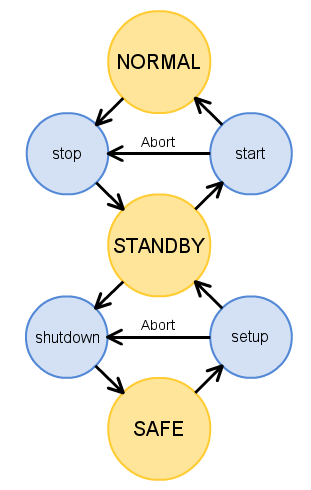
\includegraphics[scale=0.5]{pictures/mast.png}
	\caption{MAST}
	\vspace{-100pt}
	\end{center}
\end{wrapfigure}
For the Agile/Grid Manufacturing project is a State Machine designed. This State Machine consist of states and transitions. Transitions which set the State Machine to an higher state, has also an abort state to return. The State Machine is intended to control the hardware.
\subsection{States}
The State Machine will have three states:
\begin{itemize}
\item \textbf{Safe} I.e. safe for an human.
\item \textbf{Standby} I.e. the machine will be ready to run, but isn’t running.
\item \textbf{Normal} I.e. the machine is in progress.
\end{itemize}
\newpage
\subsection{Transitions}
Between the states there are transition. Transitions can be regarded as state, 'transition states' called. The transition is called as state, because most transition needed time to execute. In this time, the state State Machine should have a state, so the transition state is used as its state. Transitions are the only way to change from a state. Transition states are responsible to set the machine correct to the next state according the state requirements.  
There are four transition states:
\begin{itemize}
\item \textbf{Setup} to change from safe to standby
\item \textbf{Shutdown} to change from standby to safe
\item \textbf{Start} to change from standby to normal
\item \textbf{Stop} to change from normal to standby
\end{itemize}

\subsection{Abort Transition}
It is possible that in a transition state the transition will be undo. This option is the abort transition. When the machine in a transition state and the transition must be aborted, the transition must stop its commands and change from state to its contrary state. 
The next aborts transitions are possible:
\begin{itemize}
\item Setup to Shutdown
\item Start to Stop
\end{itemize}

\subsection{Implementation}
The StateMachine class has a transitionMap that is used to find the transition function that belongs to the transitions state. This way, a transition function can only be called when it’s in the map. So a transition from safe to standby without going through setup is impossible. The State Machine class contains all the logic for receiving state change request and sending the state update messages to the EquipletNode. The module classes only need to implement the the transition functions. Those are module specific so the State Machine can’t define those. So it’s the programmer’s responsibility to implement the transitions properly.\cite{mast_technical_design}

\newpage
\section{MOdule STateMachine (MOST)}
The State Machine is implemented by modules. This implemented State Machine is called MOST.

\subsection{Transition states}
The transition states set the module to the next state. Each Transition must be implemented in the module, because different modules has different transition implementation.

\paragraph{Setup}This transition could be used for: calibration, preheat etc.
\paragraph{Shutdown}This transition could be used for: less power of motors, cool down etc.
\paragraph{Start}The module receive Equiplet step data to execute
\paragraph{Stop}This transition could be used to set the module on its Standby position.

\subsection{Implementation}
The modules implement the State Machine by extending the StateMachine superclass. The State Machine class has virtual transition functions that need to be implemented in the module when it extends the superclass.
\\\\
The state of the module can be changed by an changeState method which is implemented in the State Machine.

\section{The Equiplet states}
Due to the nature of the (autonomous) modules in the reconfigurable system the modules can have states that differ from one another. The Equiplet node is the central point in which all modules are known. The Equiplet itself has two states, one to monitor safety and one to monitor operation. Each state depends on the states of the modules attached to the Equiplet in its own
way.
\textbf{The safety state} indicates the level of safety and is equal to the highest actor module state.
\textbf{The operation state} indicates whether the Equiplet is able to fulfill the current task and is equal to the lowest state of the required modules. The required modules are the modules necessary tofulfill the current task as known by the hardware agent.\cite{mast_funcional_design}

\section{Missing elements}
\subsection{MAST}
The current State Machine MAST which the Modules implemented miss some required functionality. These missing have been described here.
\subsubsection{Emergency button}
A module has always an emergency button to guarantees safety. When the emergency button is pressed, the software should react on it.
\subsubsection{Errors}
Modules can break down during operation. When this happens it should not receive more tasks from the Equiplet to execute. Also its current tasks can not finish.
\subsubsection{(Re-)configuration}
The current state-machine hasn't options to switch to an position to (re-)configurate or to switch to a mode of repair. An repair would see more technical information about the hardware executions and want to reconfigure.
\subsubsection{Lock}
A human would the option to lock on a state of the State Machine such as to lock on safe or standby. Lock will means that it isn't possible to call transitions. When the human lock on safe, it guarantees that the State Machine hold the safe position.

\subsection{Equiplet control}
\subsubsection{Equiplet node}
\paragraph{Modules}The Equiplet controls one or more modules. All modules implement a State Machine, but the Equiplet must react on changes of the State Machine of the modules.
\paragraph{Equiplet Step}When a module in error, the Equiplet should to stop executing its current Equiplet step and set it on an aborted state. This option is possible, because all blackboard steps contains states. 
\\Also when a module in error there are two options:
\begin{enumerate}
\item Stop executing Equiplet steps
\item Stop executing Equiplet steps which needed the module which in error.
\end{enumerate}
In both cases, the Equiplet must react when a module in error
\subsubsection{Equiplet Agent}
The Equiplet agent must know when the Equiplet node has all modules in standby. Also when modules has an error, the Equiplet should react on it such as to schedule no more.
\subsubsection{Equiplet Step Control}
Some Equiplet has a (mostly)yellow button. This button should be needed to execute Equiplet steps by once and execute next by a press on the button.